\clearpage

\section{Расчет досягаемости геометрии}\label{main_part}

Элементы поверхности. Первым шагом алгоритма будет упрощение данных о геометрии. Упрощение сводит каждый полигон к окружности, имеющей координаты центра, нормаль и площадь, оно позволит сильно упростить расчеты того, насколько одна из поверхностей затеняет другую. Центром окружности является усредненное значение координат всех точек полигона.
\begin{equation}
	\sum_{i=0}^{n} x_i / n
\end{equation}

Нормаль вычисляется по трем любым точкам ($a$, $b$, $c$) по следующей формуле:
\begin{equation}\begin{split}
	w = {(c-a) \times (b-a)} \\
	n = w \cdot 1 / \sqrt{\sum_{i=0}^{n} {w_i^2}}
\end{split}\end{equation}

Площадь треугольника вычислим по формуле Герона.
\begin{equation}\begin{split}
	p= {{a+b+c}\over{2}} \\
	S=\sqrt{p(p-a)(p-b)(p-c)}
\end{split}\end{equation}

\begin{figure}[h]
	\center
	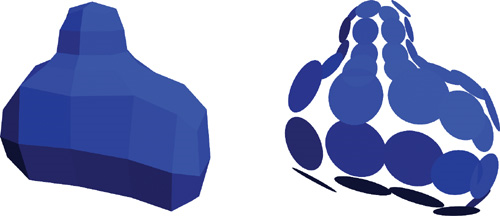
\includegraphics[width=0.5\textwidth]{14_ambient_occlusion_02}
	\caption{Перевод полигонов в диски той же площади}\label{fig:ao02}
\end{figure}
Ambient occlusion -- полезная техника для затенения объектов, которая используется в современной графике. Благодаря ambient occlusion получаются мягкие тени за счет затемнения поверхностей, которые частично видны с некоторой внешней точки. Эта техника также включает в себя расчет коэффициента досягаемости полигона к окружению, или, другими словами, число обратное числу пересечений его с другими полигонами в полусфере перед первым.

Досягаемость для каждого элемента может быть вычислена, как 1 минус доля затенения этого жлемента остальными. Быдем называть элемент, на который падает тень ресивером, а элемент бросающий тень  -- эммитером. Для расчетов количества тени, которая бросается эммитером на ресивер используется формула, основанная на телесном угле для ориентированного диска 


\begin{equation}
	1-{{r\cos{\Theta_E \max(1, 4\cos{\Theta_R})}}\over{\sqrt{{A\over\pi} + r^2}}}
	\label{em_rec}
\end{equation}
Где $А$ -- площадь эммитера\\
$E$ -- эммитер\\
$R$ -- ресивер\\
$RE$ -- отрезок, соединяющий центры дисков\\
$r$ -- длина отрезка RE, расстояние между дисками\\
$\Theta_R$ -- угол между нормалью ресивера и отрезком ER\\
$\Theta_E$ -- угол между нормалью эммитера и отрезком ER\\

\begin{figure}[h]
	\center
	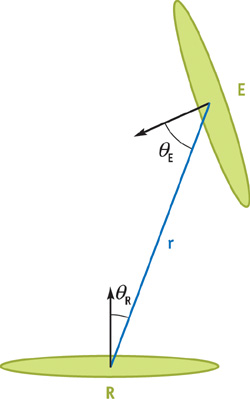
\includegraphics[width=0.3\textwidth]{14_ambient_occlusion_03}
	\caption{визуализация расположения эммитера и ресивера и эелементов уравнения \ref{em_rec}}\label{fig:ao03}
\end{figure}


